% Neural network diagram
% Made with Xematics. Positions are in px (1 px = 0.75 pt), as in the SVG export.
\documentclass[tikz, border=4pt]{standalone}
\definecolor{xm1}{HTML}{FFFFFF}
\definecolor{xm2}{HTML}{A6A6A6}
\definecolor{xm3}{HTML}{D9D9D9}
\definecolor{xm4}{HTML}{000000}
\definecolor{xm5}{HTML}{4D4D4D}
\definecolor{xm6}{HTML}{595959}
\begin{document}
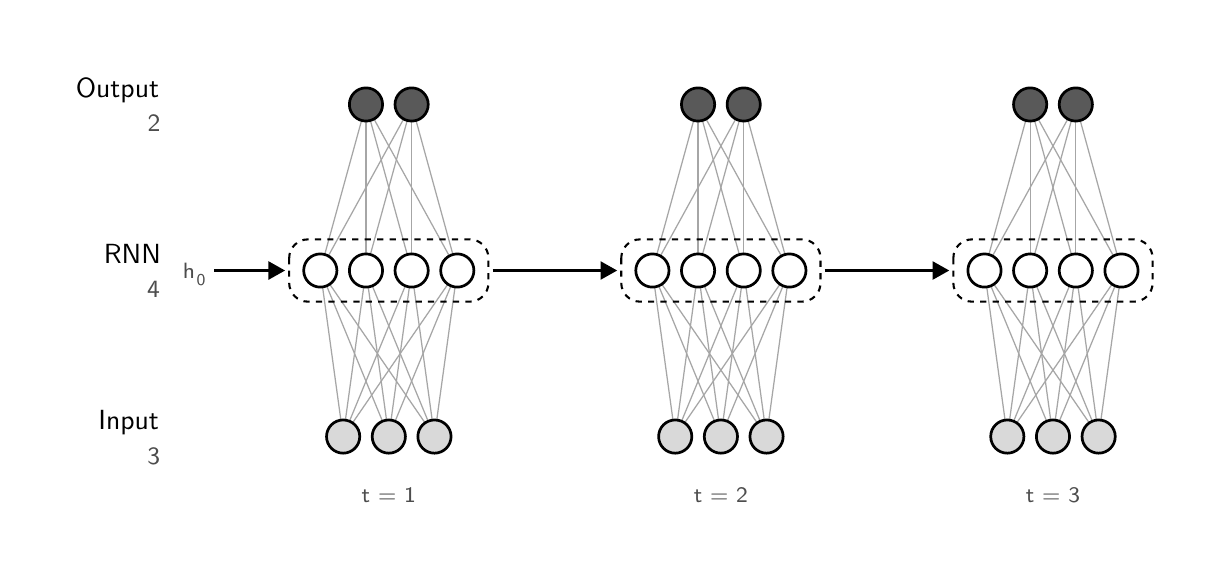
\begin{tikzpicture}[x=0.75pt, y=-0.75pt]
  \tikzset{
    xm edge cpsdym/.style={draw=xm2, line width=0.45pt},
    xm node 1gh9v2q/.style={fill=xm3, draw=xm4, line width=0.98pt},
    xm state 1y86nii/.style={draw=xm4, line width=0.98pt},
    xm state 7njxta/.style={fill=xm4, line join=round},
    xm text xm5/.style={text=xm5, inner sep=0},
    xm frame anihxq/.style={draw=xm4, line width=0.75pt, dash pattern=on 2.25pt off 2.25pt, rounded corners=6.75pt},
    xm node 1g3srx0/.style={fill=xm1, draw=xm4, line width=0.98pt},
    xm node 1h1hhtb/.style={fill=xm6, draw=xm4, line width=0.98pt},
    xm text xm4/.style={text=xm4, inner sep=0},
  }
  \fill[xm1] (0,0) rectangle (563.99,253.31);
  % Diagram
  \path[xm edge cpsdym] (150.9,189.07) -- (142.08,124.93);
  \path[xm edge cpsdym] (153.08,189.07) -- (161.9,124.93);
  \path[xm edge cpsdym] (155.04,189.6) -- (181.94,124.4);
  \path[xm edge cpsdym] (156.52,190.41) -- (202.46,123.59);
  \path[xm edge cpsdym] (170.94,189.6) -- (144.04,124.4);
  \path[xm edge cpsdym] (172.9,189.07) -- (164.08,124.93);
  \path[xm edge cpsdym] (175.08,189.07) -- (183.9,124.93);
  \path[xm edge cpsdym] (177.04,189.6) -- (203.94,124.4);
  \path[xm edge cpsdym] (191.46,190.41) -- (145.52,123.59);
  \path[xm edge cpsdym] (192.94,189.6) -- (166.04,124.4);
  \path[xm edge cpsdym] (194.9,189.07) -- (186.08,124.93);
  \path[xm edge cpsdym] (197.08,189.07) -- (205.9,124.93);
  \path[xm edge cpsdym] (310.9,189.07) -- (302.08,124.93);
  \path[xm edge cpsdym] (313.08,189.07) -- (321.9,124.93);
  \path[xm edge cpsdym] (315.04,189.6) -- (341.94,124.4);
  \path[xm edge cpsdym] (316.52,190.41) -- (362.46,123.59);
  \path[xm edge cpsdym] (330.94,189.6) -- (304.04,124.4);
  \path[xm edge cpsdym] (332.9,189.07) -- (324.08,124.93);
  \path[xm edge cpsdym] (335.08,189.07) -- (343.9,124.93);
  \path[xm edge cpsdym] (337.04,189.6) -- (363.94,124.4);
  \path[xm edge cpsdym] (351.46,190.41) -- (305.52,123.59);
  \path[xm edge cpsdym] (352.94,189.6) -- (326.04,124.4);
  \path[xm edge cpsdym] (354.9,189.07) -- (346.08,124.93);
  \path[xm edge cpsdym] (357.08,189.07) -- (365.9,124.93);
  \path[xm edge cpsdym] (470.9,189.07) -- (462.08,124.93);
  \path[xm edge cpsdym] (473.08,189.07) -- (481.9,124.93);
  \path[xm edge cpsdym] (475.04,189.6) -- (501.94,124.4);
  \path[xm edge cpsdym] (476.52,190.41) -- (522.46,123.59);
  \path[xm edge cpsdym] (490.94,189.6) -- (464.04,124.4);
  \path[xm edge cpsdym] (492.9,189.07) -- (484.08,124.93);
  \path[xm edge cpsdym] (495.08,189.07) -- (503.9,124.93);
  \path[xm edge cpsdym] (497.04,189.6) -- (523.94,124.4);
  \path[xm edge cpsdym] (511.46,190.41) -- (465.52,123.59);
  \path[xm edge cpsdym] (512.94,189.6) -- (486.04,124.4);
  \path[xm edge cpsdym] (514.9,189.07) -- (506.08,124.93);
  \path[xm edge cpsdym] (517.08,189.07) -- (525.9,124.93);
  \path[xm edge cpsdym] (143.11,109.29) -- (160.87,44.71);
  \path[xm edge cpsdym] (144.85,109.99) -- (181.14,44.01);
  \path[xm edge cpsdym] (162.99,109) -- (162.99,45);
  \path[xm edge cpsdym] (165.11,109.29) -- (182.87,44.71);
  \path[xm edge cpsdym] (182.87,109.29) -- (165.11,44.71);
  \path[xm edge cpsdym] (184.99,109) -- (184.99,45);
  \path[xm edge cpsdym] (203.14,109.99) -- (166.85,44.01);
  \path[xm edge cpsdym] (204.87,109.29) -- (187.11,44.71);
  \path[xm edge cpsdym] (303.11,109.29) -- (320.87,44.71);
  \path[xm edge cpsdym] (304.85,109.99) -- (341.14,44.01);
  \path[xm edge cpsdym] (322.99,109) -- (322.99,45);
  \path[xm edge cpsdym] (325.11,109.29) -- (342.87,44.71);
  \path[xm edge cpsdym] (342.87,109.29) -- (325.11,44.71);
  \path[xm edge cpsdym] (344.99,109) -- (344.99,45);
  \path[xm edge cpsdym] (363.14,109.99) -- (326.85,44.01);
  \path[xm edge cpsdym] (364.87,109.29) -- (347.11,44.71);
  \path[xm edge cpsdym] (463.11,109.29) -- (480.87,44.71);
  \path[xm edge cpsdym] (464.85,109.99) -- (501.14,44.01);
  \path[xm edge cpsdym] (482.99,109) -- (482.99,45);
  \path[xm edge cpsdym] (485.11,109.29) -- (502.87,44.71);
  \path[xm edge cpsdym] (502.87,109.29) -- (485.11,44.71);
  \path[xm edge cpsdym] (504.99,109) -- (504.99,45);
  \path[xm edge cpsdym] (523.14,109.99) -- (486.85,44.01);
  \path[xm edge cpsdym] (524.87,109.29) -- (507.11,44.71);
  \path[xm node 1gh9v2q] (151.99,197) circle[radius=8];
  \path[xm node 1gh9v2q] (173.99,197) circle[radius=8];
  \path[xm node 1gh9v2q] (195.99,197) circle[radius=8];
  \path[xm node 1gh9v2q] (311.99,197) circle[radius=8];
  \path[xm node 1gh9v2q] (333.99,197) circle[radius=8];
  \path[xm node 1gh9v2q] (355.99,197) circle[radius=8];
  \path[xm node 1gh9v2q] (471.99,197) circle[radius=8];
  \path[xm node 1gh9v2q] (493.99,197) circle[radius=8];
  \path[xm node 1gh9v2q] (515.99,197) circle[radius=8];
  \path[xm state 1y86nii] (223.99,117) -- (276.99,117);
  \path[xm state 7njxta] (283.99,117) -- (275.99,121.5) -- (275.99,112.5) -- cycle;
  \path[xm state 1y86nii] (383.99,117) -- (436.99,117);
  \path[xm state 7njxta] (443.99,117) -- (435.99,121.5) -- (435.99,112.5) -- cycle;
  \path[xm state 1y86nii] (89.99,117) -- (116.99,117);
  \path[xm state 7njxta] (123.99,117) -- (115.99,121.5) -- (115.99,112.5) -- cycle;
  \node[xm text xm5, font=\sffamily\fontsize{8.25}{9.9}\selectfont, anchor=base] at (77.74,121) {h};
  \node[xm text xm5, font=\sffamily\fontsize{5.94}{7.13}\selectfont, anchor=base] at (83.49,124.08) {0};
  \path[xm frame anihxq] (125.99,102) rectangle ++(96,30);
  \path[xm node 1g3srx0] (140.99,117) circle[radius=8];
  \path[xm node 1g3srx0] (162.99,117) circle[radius=8];
  \path[xm node 1g3srx0] (184.99,117) circle[radius=8];
  \path[xm node 1g3srx0] (206.99,117) circle[radius=8];
  \path[xm frame anihxq] (285.99,102) rectangle ++(96,30);
  \path[xm node 1g3srx0] (300.99,117) circle[radius=8];
  \path[xm node 1g3srx0] (322.99,117) circle[radius=8];
  \path[xm node 1g3srx0] (344.99,117) circle[radius=8];
  \path[xm node 1g3srx0] (366.99,117) circle[radius=8];
  \path[xm frame anihxq] (445.99,102) rectangle ++(96,30);
  \path[xm node 1g3srx0] (460.99,117) circle[radius=8];
  \path[xm node 1g3srx0] (482.99,117) circle[radius=8];
  \path[xm node 1g3srx0] (504.99,117) circle[radius=8];
  \path[xm node 1g3srx0] (526.99,117) circle[radius=8];
  \path[xm node 1h1hhtb] (162.99,37) circle[radius=8];
  \path[xm node 1h1hhtb] (184.99,37) circle[radius=8];
  \path[xm node 1h1hhtb] (322.99,37) circle[radius=8];
  \path[xm node 1h1hhtb] (344.99,37) circle[radius=8];
  \path[xm node 1h1hhtb] (482.99,37) circle[radius=8];
  \path[xm node 1h1hhtb] (504.99,37) circle[radius=8];
  \node[xm text xm5, font=\sffamily\fontsize{8.25}{9.9}\selectfont, anchor=base] at (173.99,228.66) {t = 1};
  \node[xm text xm5, font=\sffamily\fontsize{8.25}{9.9}\selectfont, anchor=base] at (333.99,228.66) {t = 2};
  \node[xm text xm5, font=\sffamily\fontsize{8.25}{9.9}\selectfont, anchor=base] at (493.99,228.66) {t = 3};
  \node[xm text xm4, font=\sffamily\fontsize{9.75}{11.7}\selectfont, anchor=base] at (48.67,193.47) {Input};
  \node[xm text xm5, font=\sffamily\fontsize{9}{10.8}\selectfont, anchor=base] at (60.79,210.23) {3};
  \node[xm text xm4, font=\sffamily\fontsize{9.75}{11.7}\selectfont, anchor=base] at (50.45,113.47) {RNN};
  \node[xm text xm5, font=\sffamily\fontsize{9}{10.8}\selectfont, anchor=base] at (60.62,130.23) {4};
  \node[xm text xm4, font=\sffamily\fontsize{9.75}{11.7}\selectfont, anchor=base] at (43.25,33.47) {Output};
  \node[xm text xm5, font=\sffamily\fontsize{9}{10.8}\selectfont, anchor=base] at (60.83,50.23) {2};
\end{tikzpicture}
\end{document}
